\chapter{Dynamic Causal Modelling for resting state fMRI \label{Chap:DCM_rsfmri}}

This chapter provides an extension to the framework of Dynamic Causal Modelling (DCM) for modelling intrinsic dynamics of a resting state network \cite{rsDCM2014,rsDCM2015}. This DCM estimates the effective connectivity among coupled populations of neurons, which subtends the observed functional connectivity in the frequency domain. We refer to this as spectral DCM (spDCM).

\section{Theoretical background}
Spectral DCM uses a neuronally plausible power-law model of the coupled dynamics of neuronal populations to generate complex cross spectra among measured responses. Spectral DCM is distinct from stochastic DCM (sDCM) \cite{stocDCM2011} as it eschews the estimation of random fluctuations in (hidden) neural states; rendering spectral DCM essentially deterministic in nature. These models are similar to conventional deterministic DCM for fMRI \cite{dcm} but model endogenous activity that would reproduce the functional connectivity (correlations) observed in resting state fMRI. DCMs for resting state data are also slightly simpler; given that most resting state designs compare groups of subjects (e.g. patient cohorts vs. controls), spDCMs do not usually require the bilinear term (accounting for condition-specific effects on effective connection strengths). In other words, spectral DCM is intended to simply compare endogenous coupling between groups of subjects (e.g. patients vs. healthy controls).

In modelling resting state activity, it is necessary to augment the ordinary differential equations used in standard DCM, with a stochastic term to model endogenous neuronal fluctuations. This renders the equations of the motion stochastic. The stochastic generative model for the resting state fMRI time series, like any other DCM, comprises of two equations: the Langevin form of evolution equation (motion) is written as:

\begin{equation}\label{spdcm_eq1}
\dot{z}= f(z,u,\theta)+ v
\end{equation}
and the observation equation, which is a static nonlinear mapping from the hidden physiological states in Eq.~\ref{spdcm_eq1} to the observed BOLD activity and is written as:
\begin{equation}\label{spdcm_eq2}
y= h(z,u,\phi)+ e
\end{equation}
where $\dot{z}$ is the rate in change of the neuronal states $z$, $\theta$ are unknown parameters (i.e. the effective connectivity) and $v$ (resp. $e$) is the stochastic process -- called the state noise (resp. the measurement or observation noise) -- modelling the random neuronal fluctuations that drive the resting state activity.  In the observation equations, $\phi$ are the unknown parameters of the (haemodynamic) observation function and $u$ represents any exogenous (or experimental) inputs -- that are usually absent in resting state designs. For resting state activity, Eq.~\ref{spdcm_eq1} takes on a very simple linear form:
\begin{equation}\label{spdcm_eq3}
\dot{z}= Az + Cu + v
\end{equation}
where $A$ is the Jacobian describing the behaviour -- i.e. the effective connectivity -- of the system near its stationary point ($f(z_{o})=0$) in the absence of the fluctuations $v$. It is to be noted that we can still include exogenous (or experimental) inputs, $u$  in our model. These inputs drive the hidden states -- and are usually set to zero in resting state models. It is perfectly possible to have external, (non-modulatory) stimuli, as in the case of conventional functional neuroimaging studies. For example, in \cite{dcm} we used an attention to visual motion paradigm to illustrate this point.

Inverting the stochastic DCM of the form given by Eq.~\ref{spdcm_eq3} in the time domain, which includes state noise, is rather complicated because such models require estimation of not only the model parameters (and any hyperparameters that parameterise the random fluctuations), but also the hidden states, which become random (probabilistic) variables. Hence the unknown quantities to be estimated under a stochastic DCM are  $\psi=\{z,\phi,\theta,\sigma\}$, where $\sigma$ refers to any hyperparameters (precisions or inverse covariances) defining the neuronal fluctuations. In terms of temporal characteristics, the hidden states are time-variant, whereas the model parameters (and hyperparameters) are time-invariant. There are various variational schemes in literature that can invert such models. For example, dynamic expectation maximization (DEM) \cite{karl_DEM} and generalized filtering (GF) \cite{karl_generalised_filtering}.

Although the stochastic models in  Eq.~\ref{spdcm_eq1} and their inversion in time domain provide a useful means to estimate effective connectivity they also require us to estimate hidden states. This poses a difficult inverse problem that is computationally demanding; especially when the number of hidden states becomes large. To finesse this problem, we furnish a constrained inversion of the stochastic model by parameterising the neuronal fluctuations. This parameterisation also provides an opportunity to compare parameters encoding the neuronal fluctuations among groups. The parameterisation of endogenous fluctuations means that the states are no longer probabilistic; hence the inversion scheme is significantly simpler, requiring estimation of only the parameters (and hyperparameters) of the model.

Spectral DCM simply estimates the time-invariant parameters of their cross spectra. In other words, while stochastic DCMs model the observed BOLD timeseries of each node, spectral DCMs model the observed functional connectivity between nodes. Effectively, this is achieved by replacing the original timeseries with their second-order statistics (i.e., cross spectra), under stationarity assumptions. This means, instead of estimating time varying hidden states, we are estimating their covariance, which does not change with time. This means we need to estimate the covariance of the random fluctuations; where a scale free (power law) form for the state noise (resp. observation noise) that can be motivated from previous work on neuronal activity:
\begin{eqnarray}\label{spdcm_eq4}
& g_{v}(\omega,\theta) & = \alpha_{v}\omega^{-\beta_{v}}\\ \nonumber
& g_{e}(\omega,\theta) & = \alpha_{e}\omega^{-\beta_{e}}
\end{eqnarray}
Here, $\{\alpha,\beta\}\subset \theta$ are the parameters controlling the amplitudes and exponents of the spectral density of the neural fluctuations. This models neuronal noise with a generic $1/f^{\gamma}$ spectra, which characterizes fluctuations in systems that are at nonequilibrium steady-state. Using the model parameters, $\theta \supseteq \{A,C,\alpha, \beta\}$, we can simply generate the expected cross spectra:
\begin{eqnarray}\label{spdcm_eq5}
& y & = \kappa \ast v + e\\ \nonumber
& \kappa & = \partial_z h \mathrm{exp} (t \partial_z f ) \\ \nonumber
& g_{y}(\omega,\theta) & = |K(\omega)|^2 g_{v}(\omega,\theta) + g_{e}(\omega,\theta)
\end{eqnarray}
where $K(\omega)$ is the Fourier transform of the system's (first order) Volterra kernels  $\kappa$, which are a function of the Jacobian or effective connectivity. The unknown quantities $\psi=\{\phi,\theta,\sigma\}$ of this deterministic model can now be estimated using standard Variational Laplace procedures \cite{karl_vb_laplace}. Here $g_{y} (\omega,\theta)$ represents the predicted cross spectra that can be estimated, for example, using autoregressive (AR) model. Specifically, we use a fourth-order autoregressive model to ensure smooth sample cross spectra of the sort predicted by the generative model. The frequencies usually considered for fMRI range from 1/128 Hz to 0.1 Hz in 32 evenly spaced frequency bins.

\section{Practical example}

Data used for this example can be downloaded from the SPM website. This dataset\footnote{Resting state DCM dataset: \url{http://www.fil.ion.ucl.ac.uk/spm/data/spDCM/}} consists of an exemplar subject from the full dataset available from the FC1000 project website\footnote{``1000 Functional Connectomes'' Project,: \url{http://fcon_1000.projects.nitrc.org/fcpClassic/FcpTable.html}} and was used in \cite{rsDCM2015} to interrogate the information integration in default mode network (DMN) -- a distinct brain system that is activated when an individual engages in introspection like mindwandering or daydreaming. The DMN comprises part of the medial prefrontal cortex (mPFC), posterior cingulate cortex (PCC) and parts of inferior parietal lobe and superior frontal regions.

The archive contains the smoothed, spatially normalised, realigned, slice-time corrected images in the directory \texttt{func}. The directory \texttt{anat} contains a spatially normalised T1 structural image and the directory \texttt{GLM} contains the file \texttt{rp\_rest0000.txt} containing six head motion parameters. All preprocessing took place using SPM12.

\subsection{Defining the GLM}
First, we need to set up the GLM analysis and extract our time series from the results. For resting state fMRI because there is no task so first we need to generate \texttt{SPM.mat} so that we can extract the time series. This can be done by following the steps below.

Let's set up a batch that will specify the model and estimate it.

\begin{enumerate}
 \item The analysis directory you have downloaded should include:
 \begin{enumerate}
  \item A directory named \texttt{func}, which includes the preprocessed fMRI volumes.
  \item A directory named \texttt{anat}, which includes a normalised T1 structural volume.
  \item A directory named \texttt{GLM}, which include file \texttt{rp\_rest0000.txt} containing the movement regressors from the realignment step.
 \end{enumerate}
 \item In \matlab\ type
\begin{verbatim}
>> cd GLM
>> spm fmri
\end{verbatim}
 \item From the main SPM window, click on the \textsc{Batch} button.
 \item From the SPM menu at the top of the Batch Editor, select ``Stats $>$ fMRI model specification''.
 \item Click \textsc{Directory} and choose the \texttt{GLM} directory that you made above.
 \item \textsc{Units for design} [\textsc{scans}]
 \item \textsc{Interscan interval} [2]
 \item Click \textsc{Data \& Design}, Choose \textsc{New "Subject/Session"}
 \item Click \textsc{Scans} and choose all the functional scans \texttt{swrestxxxx.img}. There should be 175 \texttt{*.img} files.
 \item From the SPM menu at the top of the Batch Editor, select ``Stats $>$ model estimation''.
 \item For \textsc{Select SPM.mat}, click on the \textsc{Dependency} button and choose the proposed item (the output from the previous module).
 \item You should now be able to press the \textsc{Run} green arrow at the top of the Batch Editor window. This will specify and estimate the GLM.
\end{enumerate}

We will also need to extract signal from CSF and white matter (WM) to be used as confound. Here is a step-by-step example for extracting the WM (Pons) time series which we will use as one of the nuisance variable:

\begin{enumerate}
 \item From the main SPM window, click on the \textsc{Batch} button.
 \item From the SPM menu at the top of the Batch Editor, select ``Util $>$ Volume of interest''
 \item Select the \texttt{SPM.mat} file (generated during the previous section).
 \item Adjust data: \texttt{NaN}
 \item Which session: \texttt{1}
 \item Name of VOI: \texttt{WM}
 \item Select 'Region(s) of Interest' $>$ Sphere
 \item Centre: \texttt{[0 -24 -33]}
 \item VOI radius (mm): e.g.\texttt{6} mm
 \item Select 'Movement of Centre' $>$ Fixed
 \item Select 'Region of Interest' $>$ Mask Image
 \item Image file: select \texttt{mask.nii} (in \texttt{GLM} folder)
 \item Expression: \texttt{i1\&i2}
 \item Now you should be able to press the green arrow button. This would extract the WM time series and save this as  \texttt{VOI\_WM\_1.mat} in the working directory.
\end{enumerate}

Do the same thing with to extract CSF (from one of the ventricles) signal with a sphere centred on \texttt{[0 -40 -5]}. This will create files \texttt{VOI\_CSF\_1.mat}. Next we need to adjust the SPM with the covariates. Do the following procedure:
\begin{enumerate}
 \item From the main SPM window, click on the \textsc{Batch} button.
 \item From the SPM menu at the top of the \textsc{Batch Editor}, select ``Stats $>$ fMRI model specification''.
 \item Click Directory and choose the \texttt{GLM} directory that you made above.
 \item \textsc{Units for design} [\textsc{scans}]
 \item \textsc{Interscan interval} [2]
 \item Click \textsc{Data \& Design}, Choose \textsc{New "Subject/Session"}
  \item Click \textsc{Scans} and choose all the functional scans \texttt{swrestxxxx.img}. There should be 175 \texttt{*.img} files.
 \item Click on Multiple Regressors. And then select the  \texttt{VOI\_CSF\_1.mat}t, \texttt{VOI\_WM\_1.mat} and \texttt{rp\_rest000.txt}. Leave the rest of the fields as default. 
 \item From the SPM menu at the top of the Batch Editor, select ``Stats $>$ model estimation''.
 \item For \textsc{Select SPM.mat}, click on the \textsc{Dependency} button and choose the proposed item (the output from the previous module).
 \item You should now be able to press the \textsc{Run} green arrow at the top of the Batch Editor window (press 'continue' when asked for overwriting existing \textsc{SPM.mat} file). This will specify and estimate the GLM.
\end{enumerate}

\subsection{Extracting time series}

Once you have specified and estimated the GLM, here is now a step-by-step example for extracting the PCC time series:
\begin{enumerate}
 \item From the main SPM window, click on the \textsc{Batch} button.
 \item From the SPM menu at the top of the Batch Editor, select ``Util $>$ Volume of interest''
 \item Select the \texttt{SPM.mat} file (generated during the previous section).
 \item Adjust data: \texttt{NaN}
 \item Which session: \texttt{1}
 \item Name of VOI: \texttt{PCC}
 \item Select 'Region(s) of Interet' $>$ Sphere
 \item Centre: \texttt{[0 -52 26]}
 \item VOI radius(mm): e.g.\texttt{ 8} mm
 \item Select 'Movement of Centre' $>$ Fixed
 \item Select 'Region of Interest' $>$ Mask Image
 \item Image file: select \texttt{mask.nii} (in \texttt{GLM} folder)
 \item Expression: \texttt{i1\&i2}
 \item Now you should be able to press the green arrow button. This would extract the WM time series and save this as  \texttt{VOI\_CSF\_1.mat} in the working directory.
\end{enumerate}
SPM now computes the first principal component of the time series from all voxels included in the sphere. The result is stored (together with the original time series) in a file named \texttt{VOI\_PCC\_1.mat} in the working directory (the ``1'' refers to session 1). Do the same for the rest of the VOIs: mPFC (\texttt{[3 54 -2]}), LIPC ({[-50 -63 32]}) and RIPC (\texttt{[48 -69 35]}).

\subsection{Specifying and estimating the DCM}

Now we have extracted the time series, we are ready to build the DCM. We will look at a simplified version of the model described in \cite{rsDCM2015}.  In our example here, we will model a fully connected system comprising PCC, mPFC and bilateral IPC. This DCM is shown schematically in Figure~\ref{spdcm_full}, and can be made as follows:
\begin{enumerate}
 \item Press the large \texttt{Dynamic Causal Modelling} button.
 \item Choose \textsc{specify}.
 \item Select the \texttt{SPM.mat} file you just created when specifying the GLM.
 \item \texttt{DCM\_???.mat}: e.g. \texttt{DMN}.
 \item Select all VOIs in order \texttt{VOI\_PCC\_1}, \texttt{VOI\_mPFC\_1}, \texttt{VOI\_LIPC\_1} and  \texttt{VOI\_RIPC\_1}.
 \item Specify slice timings for each area. The default values are set to the last slice of the data, which was the default in the original DCM version. For sequential (as opposed to interleaved) data, this modelling option allows to use DCM in combination with any TR (slice timing differences). Here, we proceed with the default values.
\item Enter \texttt{0.04} for ``Echo Time, TE[s]''.
\item Define the fully connected model. Your connectivity matrix should look like the one in See Figure~\ref{spdcm_Fig1}.
\end{enumerate}
A polite ``Thank you'' completes the model specification process. A file called \texttt{DCM\_DMN.mat} will have been generated.

You can now estimate the model parameters, either by pressing the DCM button again and choosing \textsc{estimate (cross-spectra)}, or by typing
\begin{verbatim}
>> spm_dcm_estimate('DCM_DMN');
\end{verbatim}
from the \matlab\ command line.

Once this is completed, you can review the results as follows:
\begin{enumerate}
\item Press the DCM button.
\item Choose \textsc{review}.
\item Select \texttt{DCM\_DMN.mat}
\end{enumerate}

By clicking ``review...'' you can now select from multiple options, e.g. you can revisit the fit of the model (``Cross-spectra (BOLD)''), shown in Figure~\ref{spdcm_Fig2} or look at the parameter estimates for the endogenous coupling (``Coupling (A)'') as shown in Figure~\ref{spdcm_Fig3}. Of course, you can also explore the model results at the level of the \matlab\ command line by loading the model and inspecting the parameter estimates directly. These can be found in \texttt{DCM.Ep.A} (endogenous coupling) and  \texttt{DCM.Ep.a }(neuronal parameters).

\begin{figure}[ht]
\begin{center}
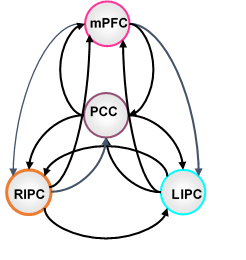
\includegraphics[width=100mm]{dcm_rs/dcm_mod_full}
\caption{\em DCM with fully connected model.\label{spdcm_full}}
\end{center}
\end{figure}


\begin{figure}
\begin{center}
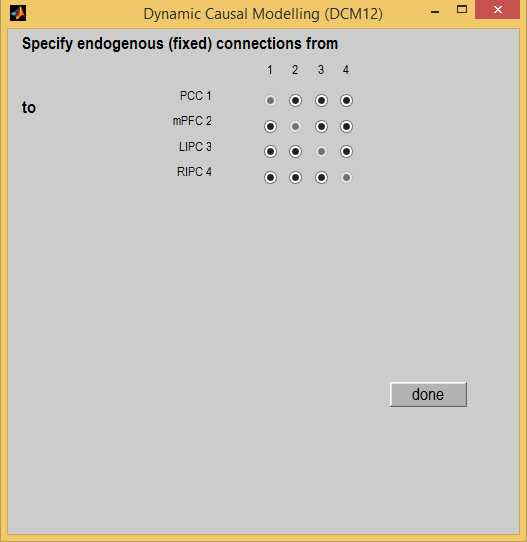
\includegraphics[width=100mm]{dcm_rs/Fig1}
\caption{\em Specification of model depicted in Fig~\ref{spdcm_Fig1}. Filled circles define the structure of the extrinsic connections A such that all circles are filled since we are using a fully connected model here.
\label{spdcm_Fig1}}
\end{center}
\end{figure}

\begin{figure}[ht]
\begin{center}
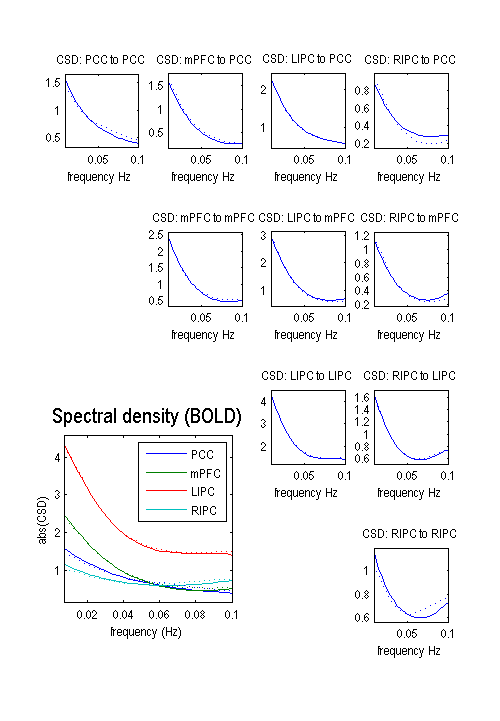
\includegraphics[width=140mm]{dcm_rs/Fig2}
\caption{\em Plot of predicted and observed cross spectral densities after convergence in Fig~\ref{spdcm_Fig2}. The dotted lines are measured cross spectra and solid lines are its predictions. The lower left panel shows the self cross spectra for the four regions. The rest of the graphics show both self and cross spectra for the four regions.
\label{spdcm_Fig2}}
\end{center}
\end{figure}

\begin{figure}[ht]
\begin{center}
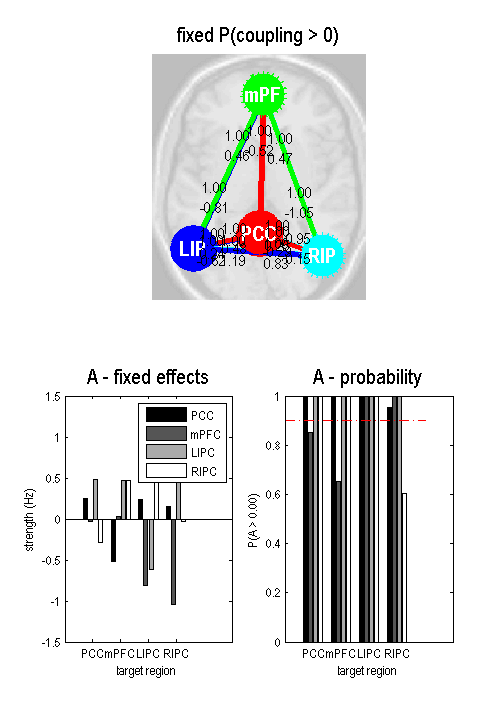
\includegraphics[width=140mm]{dcm_rs/Fig3}
\caption{\em This Fig~\ref{spdcm_Fig3} shows the estimated fixed A matrix (top and lower left panels). The posterior probabilities of these effective connectivity parameters are shown on the lower right panel. The red dashed line depicts the 95\% threshold.
\label{spdcm_Fig3}}
\end{center}
\end{figure}
